\documentclass{article}

\usepackage{graphicx}

\author{Thomas Dizon}
\title{Implementing a Software Rasterizer in C}

\begin{document}

\maketitle

\begin{figure}[h]
	\centering
	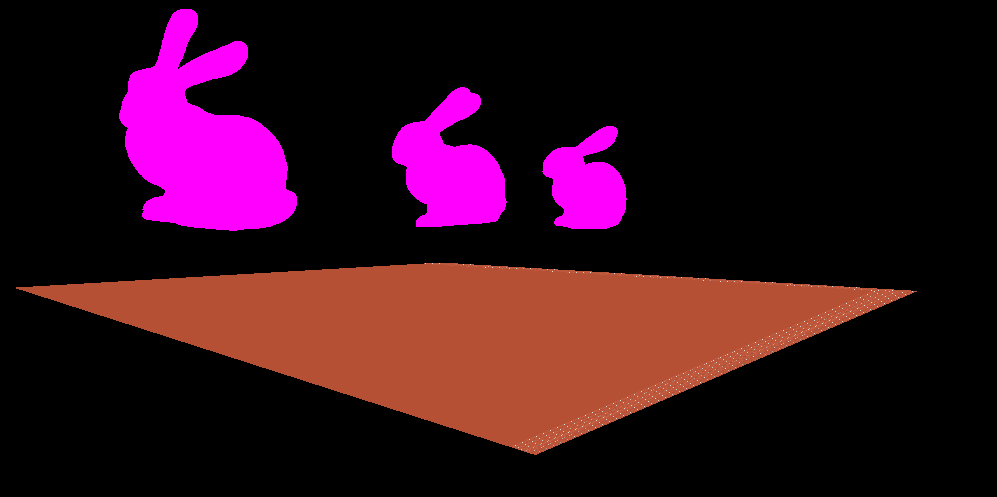
\includegraphics[width=0.6\textwidth]{scene.png}
	\caption{}
\end{figure}

\newpage

\tableofcontents

\newpage

\section{Abstract}

\section{Introduction}

\subsection{Motivation}
\subsection{What is a \textit{Software Rasterizer}?}
\subsection{Why \textit{C}?}

\section{Background}
\subsection{Algorithms}
\subsection{Math Concepts}
\subsection{Computer Graphics Concepts}

\section{System Architecture}
\subsection{Overview}
\subsection{Project Structure}
\subsection{Data Design}
\subsection{Software Design}

\section{Conclusion \& Future Work}
\subsection{What I learnt}
\subsection{A future implementation in C++}

\section{References}

\end{document}

